%!TEX root = ../thesis.tex
%*******************************************************************************
%****************************** Third Chapter **********************************
%*******************************************************************************
\chapter{PERANCANGAN SISTEM}

% **************************** Define Graphics Path **************************
\ifpdf
    \graphicspath{{Chapter3/Figs/Raster/}{Chapter3/Figs/PDF/}{Chapter3/Figs/}}
\else
    \graphicspath{{Chapter3/Figs/Vector/}{Chapter3/Figs/}}
\fi

\section{ Perancangan Sistem Kerja}
\subsection{ Skenario Yang Digunakan}
Pada bagian ini akan dibahas tentang perancangan sistem yang akan digunakan pada proyek akhir ini. Secara sederhana, proyek akhir ini terdiri atas tiga bagian yaitu perangkat pengambilan data, mekanisme komunikasi dan perangkat pengolahan data. 


\begin{figure}[ht]
 \centering
 \includegraphics[width=\textwidth]{diagramblok}
 \caption{Perancangan Sistem Kerja}
 \label{fig:diagramblok}   
\end{figure}

Seperti terlihat pada Gambar~\ref{fig:diagramblok}, fokus dari proyek akhir ini \textbf{ditandai oleh warna merah}. Perangkat pengambilan data yaitu Raspberry Pi 3 dengan berbagai sensor seperti kamera, orientasi dan GPS yang dibawa oleh sebuah Quadcopter. Mekanisme komunikasi yaitu cara pengiriman data sensor oleh perangkat pengambilan data menuju perangkat pengolahan data dimana akan digunakan MQTT yang bekerja diatas TCP/IP jaringan WiFi 2.4GHz. Perangkat pengolahan data berupa perangkat komputer dengan kemampuan komputasi tinggi dimana dilakukan proses Learning maupun Testing di dalamnya. Proses Learning dan Testing tersebut menggunakan Framework Deep Learning Caffe yang berjalan pada sistem operasi Ubuntu Linux 16.04.

\subsection{ Gambar Drone Bawa Kotak Sensor}
Lorem ipsum dolor sit amet, consectetur adipiscing elit. Nullam ante quam, varius id tincidunt in, aliquet gravida felis. Praesent vehicula risus at pulvinar mattis. Duis feugiat diam ut massa euismod mollis. Maecenas tempus nisl diam, et sodales massa pharetra ut. Duis id ipsum ut dolor tincidunt euismod vitae sed odio. Duis tincidunt lorem ac leo mattis varius. Sed mollis metus nec tempor congue. Ut imperdiet dui ut ante mollis auctor. Suspendisse sit amet scelerisque sapien, in cursus nisl. Etiam egestas tellus mi, non fringilla justo ultricies at. Praesent eget ipsum porta, fermentum lorem sit amet, suscipit ligula. Nulla porttitor finibus neque nec sodales. Orci varius natoque penatibus et magnis dis parturient montes, nascetur ridiculus mus. Maecenas auctor quam ut justo accumsan, consequat eleifend massa imperdiet. Ut dictum eleifend justo, vitae pellentesque eros porta id.

\section{ Konfigurasi Perangkat Keras Dan Lunak}
\subsection{ Spesifikasi Pengolahan Data}
Perangkat pemrosesan dalam hal ini adalah sebuah komputer yang nantinya akan menjalankan proses Deep Learning. Hal yang harus diperhatikan dalam merancang komputer untuk Deep Learning adalah bagaimana caranya agar hardware yang digunakan mampu mempercepat proses learning. Itu penting karena proses learning dapat memakan waktu dalam hitungan jam, hari bahkan bulan. Deep Learning membutuhkan proses perkalian matrix dalam jumlah sangat banyak, maka untuk mempercepatnya dapat dilakukan pengerjaan dengan mekanisme paralel processing, dimana sebuah proses akan dikerjakan oleh semua cores dari processing unit sekaligus.

Terdapat dua cara untuk menjalankan Deep Learning, CPU mode dan GPU mode. CPU memiliki kecepatan tiap core yang lebih tinggi dari GPU, namun memiliki jumlah core yang sangat sedikit dibandingkan GPU. Hal tersebut membuat menjalankan GPU mode dapat berjalan 5x lebih cepat, bahkan perbandingannya semakin besar jika kompleksitas yang dikerjakan juga semakin tinggi. Pada Tabel \ref{table:spek_pc} membandingkan jumlah core dan kecepatannya masing masing pada CPU dan GPU yang digunakan.

\begin{table}[ht]
\caption{Spesifikasi Komputer untuk Deep Learning}
\centering
\label{table:spek_pc}
\resizebox{\textwidth}{!}{%
\begin{tabular}{| c c |}
\hline 
Komponen & Tipe \\
\hline
GPU & Zotac Geforce GTX 1080 AMP Extreme Edition \\
& \textbf{2560 Cuda Cores @ 1771-1911 MHz}\\
& \textbf{GDDR5X} \\
CPU & Intel i7-6700K \\
& \textbf{4 Cores 8 Threads @ 4.0-4.2 GHz}\\
Motherboard & Asrock Z170 Extreme 4 \\
Power Supply & Seasonic G750 - 750W Gold \\
RAM & Corsair DDR4 8GB 2400 \\
HDD & WDC 1TB blue \\
Case & NZXT S340 Black-Red \\
Cooling & ID Cooling IS 60 \\
\hline 
\end{tabular} 
}
\end{table}

Walaupun pada GPU mode semua perhitungan perkalian matrix akan dibebankan pada GPU, namun tetap harus disandingkan dengan CPU yang sesuai. Hal tersebut untuk menghindari terjadinya Bottleneck pada kecepatan proses data. RAM yang digunakan juga harus minimal sama dengan RAM yang dimiliki GPU agar proses pemindahan data dari GPU ke CPU tidak terjadi Bottleneck juga.

Hal lain yang harus diperhatikan adalah ketersediaan daya yang cukup dari power supply. Power supply pada komputer memiliki standarisasi 80+ yaitu besaran efisiensi yang dapat dikeluarkan sehingga mampu menghemat daya, lebih stabil dan membuat komponen hardware, termasuk GPU yang membutuhkan daya besar, lebih tahan lama.

\subsection{ Instalasi software (cuda, cudnn)}

Lorem ipsum dolor sit amet, consectetur adipiscing elit. Nullam ante quam, varius id tincidunt in, aliquet gravida felis. Praesent vehicula risus at pulvinar mattis. Duis feugiat diam ut massa euismod mollis. Maecenas tempus nisl diam, et sodales massa pharetra ut. Duis id ipsum ut dolor tincidunt euismod vitae sed odio. Duis tincidunt lorem ac leo mattis varius. Sed mollis metus nec tempor congue. Ut imperdiet dui ut ante mollis auctor. Suspendisse sit amet scelerisque sapien, in cursus nisl. Etiam egestas tellus mi, non fringilla justo ultricies at. Praesent eget ipsum porta, fermentum lorem sit amet, suscipit ligula. Nulla porttitor finibus neque nec sodales. Orci varius natoque penatibus et magnis dis parturient montes, nascetur ridiculus mus. Maecenas auctor quam ut justo accumsan, consequat eleifend massa imperdiet. Ut dictum eleifend justo, vitae pellentesque eros porta id.

\subsection{ Perangkat pengambilan data (raspberry skematik, berapa megapiksel dengan kecepatan terbang berapa)}

Raspberry Pi merupakan sebuah Single Board Computer (SBC) yang dilengkapi dengan General Purpose Input Output (GPIO) Pin. Raspberry Pi 3 dilengkapi dengan prosesor quad-core 64-bit ARM Cortex A53 1.2 GHz, 1 GB RAM dan GPU VideoCore IV @ 300 MHz yang dirangkum pada System on Chip (SoC) Broadcom BCM2837. Raspberry Pi mampu menjalankan sistem operasi Linux tipe ARM-HF sehingga mampu untuk menjalankan bahasa pemrograman tingkat tinggi dan komputasi layaknya komputer. Fitur terbaru dalam Raspberry Pi 3 adalah kemudahan konektifitas 802.11n WiFi dan Bluetooth 4.0 yang telah tertanam dalam sistem.

\begin{figure}[ht]
 \centering
 \includegraphics[width=\textwidth]{raspi_spec}
 \caption{Beberapa Bagian Penting Raspberry Pi 3 yang Perlu Diperhatikan}
 \label{fig:raspi_spec}   
\end{figure} 

Raspberry Pi akan digunakan sebagai media pengambilan gambar dan komunikasi dengan GPS dan memanfaatkan beberapa bagian penting seperti terlihat pada Gambar~\ref{fig:raspi_spec}. Raspberry Pi mendukung dua jenis kamera yaitu RaspiCam Board yang terhubung melalui Camera Serial interface (CSI) atau Webcam yang terhubung melalui USB. Webcam dengan interfaces USB akan membebankan CPU, sedangkan dengan interfaces CSI lebih kepada pemrosesan menggunakan GPU (\citet[p.~42]{creasey2015raspberry}). Selain itu RaspiCam juga memiliki ukuran yang ringkas sehingga lebih mudah untuk dibawa dan dikemas seperti pada Gambar~\ref{fig:raspiku}

\begin{figure}[ht]
 \centering
 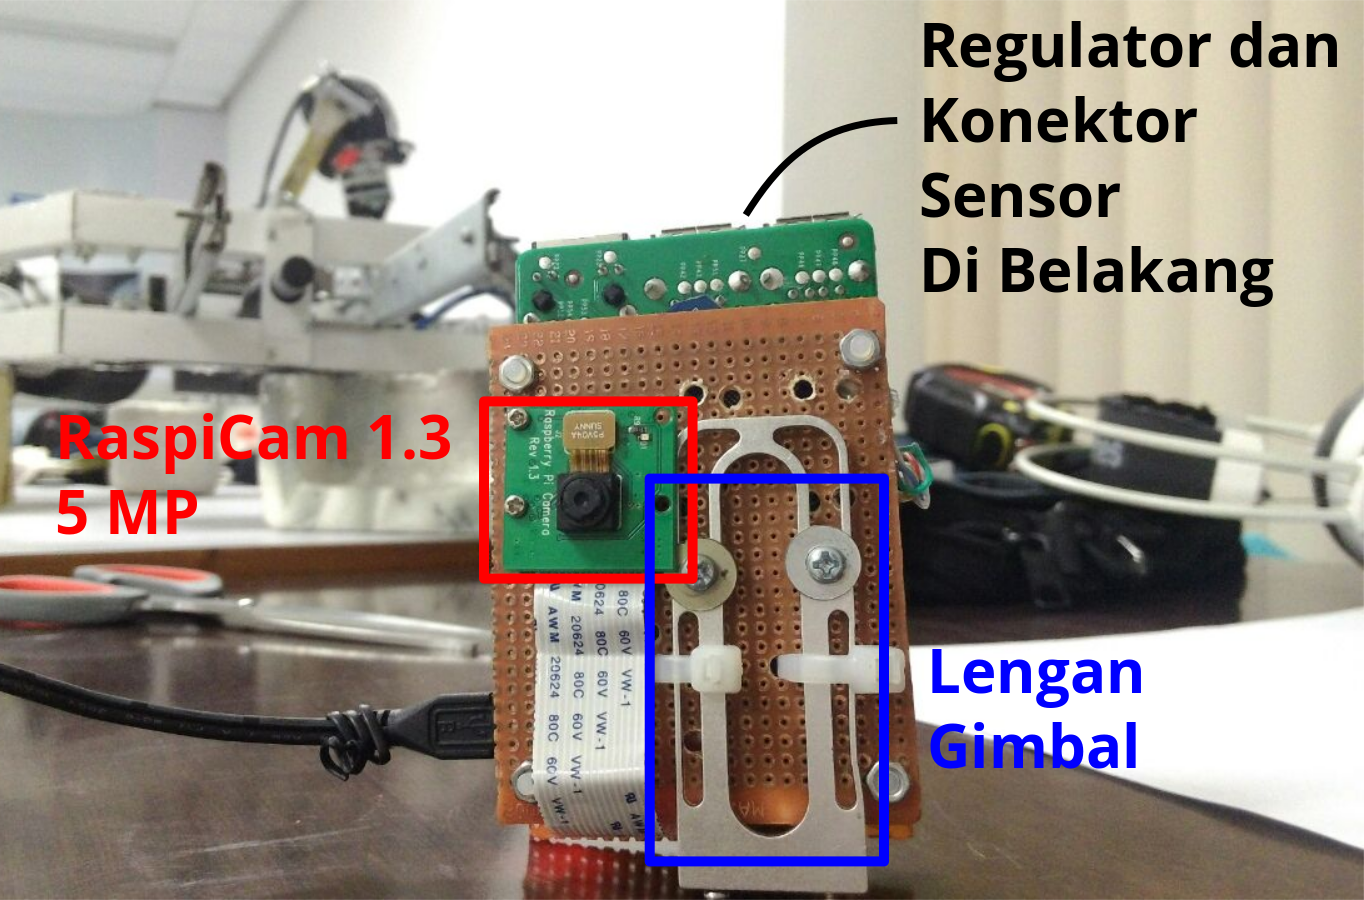
\includegraphics[width=\textwidth]{raspiku}
 \caption{Konfigurasi Raspberry Pi yang akan Digunakan}
 \label{fig:raspiku}   
\end{figure}  

Setelah dilakukan pengambilan gambar oleh kamera, yang harus dilakukan adalah pengiriman gambar dan data sensor menuju perangkat pengolahan data menggunakan protokol Message Queuing Telemetry Transport (MQTT) yang menggunakan koneksi WiFi. Komunikasi dapat dilakukan selama dalam satu jaringan dan Raspberry Pi mampu terhubung baik menggunakan built-in WiFi maupun WiFi adapter via USB. Secara sederhana, komunikasi tersebut dirancang seperti Gambar~\ref{fig:raspi}.

\begin{figure}[ht]
 \centering
 \includegraphics[width=\textwidth]{raspi}
 \caption{Perancangan Mekanisme Pengambilan Data}
 \label{fig:raspi}   
\end{figure}   

\subsection{ Komunikasi pengiriman data (gui, mqtt, mavlink)}
MQTT (Message Queuing Telemetry Transport) \cite{banks2014mqtt}, adalah sebuah protokol pengiriman pesan berbasis Client-Server Publish-Subcribe yang berjalan diatas TCP/IP. MQTT diklaim sebagai sebuah protokol yang ringan, open, sederhana dan mudah untuk diimplementasikan. Hal tersebut membuat protokol ini banyak digunakan untuk komunikasi dalam Machine to Machine (M2M) dan Internet of Things (IoT) dimana hanya memiliki resource terbatas dan bandwidth yang tidak terlalu besar. Dengan memanfaatkan kecepatan dan protokol yang ringan tersebut maka dapat dianggap hal tersebut cocok untuk digunakan sebagai pengiriman data berupa gambar dan GPS.

\begin{figure}[ht]
 \centering
 \includegraphics[width=\textwidth]{mqtt}
 \caption{Protokol MQTT yang Digunakan}
 \label{fig:mqtt}   
\end{figure}

Setidaknya dibutuhkan tiga aspek dalam menjalankan MQTT yaitu Publisher, Subcriber dan Broker. Publisher adalah client yang mengirimkan data pada suatu topik sedangkan Subcriber adalah client yang menerima data pada suatu topik. Client tersebut dapat menjadi Publisher atau Subcriber secara bergantian. Broker adalah sebuah server dimana akan menerima data yang dikirim dari Publisher dan akan dilakukan broadcast kepada Subcriber yang mengikuti topik tertentu. Subcriber hanya akan menerima data dari topik yang dia ikuti saja (subcribe). 

Protokol MQTT terdiri dari tiga yaitu Fixed Header, Variable Header dan Payload. Maximum payload dari MQTT adalah 268.435.455 Bytes atau 268 MB. Data yang dikirimkan oleh MQTT berupa String sedangkan gambar merupakan sebuah array tiga dimensi dengan rentang nilai 0-255, sehingga diperlukan konversi, salah satunya dengan \textit{encode base64}. 

\section{ Proses learning CNN    }
\subsection{ Dataset}
Dataset yang digunakan adalah PASCAL VOC 2007 \cite{Everingham10} (Pattern Analysis Statistical Modelling and Computational Learning Visual Object Classes). PASCAL VOC Project memberikan standar untuk Dataset gambar untuk pengenalan objek serta mengadakan tantangan dari 2005 hingga 2012 untuk peneliti mengembangkan algoritma deteksi objek terbaik. PASCAL VOC 2007 digunakan karena merupakan dataset yang digunakan untuk pengujian Faster R-CNN dimana memiliki 9.963 gambar dengan 24.640 objek serta menjadi baku untuk dataset tahun berikutnya. Gambartersebut terdiri dari 4952 gambar untuk testing dan 5011 gambar untuk training. Ukuran masing masing gambar berkisar 335x500 px untuk potrait dan 500x350 px untuk landscape. Berikut terdapat sebuah contoh untuk membaca sebuah dataset.

\begin{figure}[ht]
 \centering
 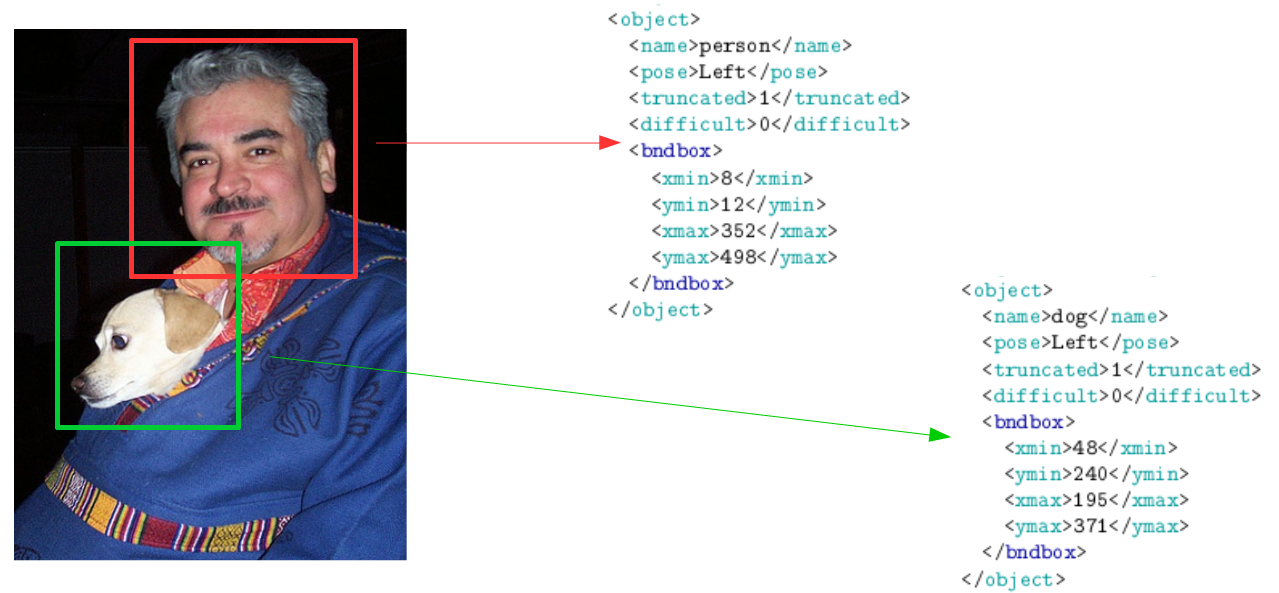
\includegraphics[width=\textwidth]{voc2007}
 \caption{Gambar000001.jpg Pada Dataset VOC2007 dan Anotasinya }
 \label{fig:voc2007}   
\end{figure}  

Gambar~\ref{fig:voc2007} merupakan salah satu foto yang digunakan pada dataset VOC2007 yang didefinisikan dengan format XML untuk memberikan data kepada Net untuk mempelajari area yang ditentukan. Yang perlu diperhatikan pada kode tersebut dimulai dari object, dimana akan didefinisikan nama, pose dan bounding box (bndbox). Bounding Box tersebut mendifinisikan area yang terdapat objek dengan nama tertentu dan berpose tertentu. Dengan diberikannya berbagai macam jenis foto yang berbeda maka komputer akan menghitung hingga didapat model persamaan tersebut.

Pengembangan selanjutnya akan digunakan dataset INRIA \cite{dalal2005histograms} dan pembuatan dataset sendiri. Dataset INRIA merupakan dataset yang berisi foto positif (terdapat manusia) atau negatif (tidak ada manusia) serta tanda (annotation) yang mendefinisikan posisi manusia.

\subsection{ Struktur Layer}
Perancangan layer untuk mendeteksi korban bencana alam diberikan sebuah fokus untuk mencari manusia terlebih dahulu. Untuk itu dirancanglah sebuah Net untuk secara khusus mendeteksi objek berupa manusia. Secara sederhana Net tersebut disajikan pada Gambar~\ref{fig:strukturcnn}.

\begin{figure}[ht]
  \centering
  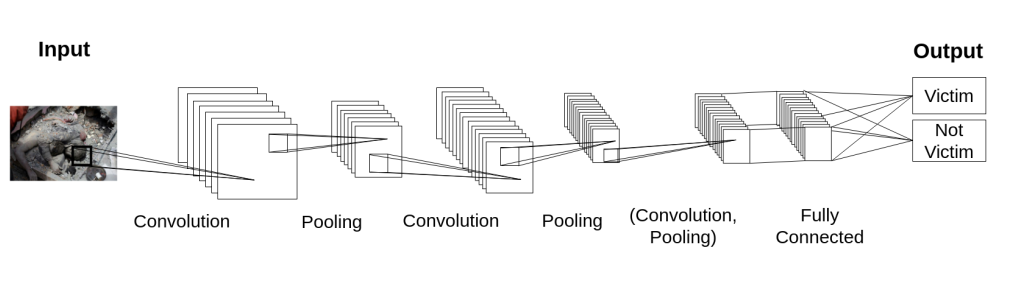
\includegraphics[width=\textwidth]{strukturcnn}
  \caption{Struktur CNN Deteksi Korban Bencana Alam}
  \label{fig:strukturcnn}
\end{figure}

Dari Net tersebut, disesuaikan dengan beberapa Net yaitu VGG16, VGG CNN M 1024 dan ZFnet. Masing masing Net selanjutnya dihubungkan pada RPN yang ada pada Faster R-CNN. Secara sederhana, Net tersebut disajikan pada Gambar~\ref{fig:struktur_rcnn}.

\begin{figure}[ht]
  \centering
  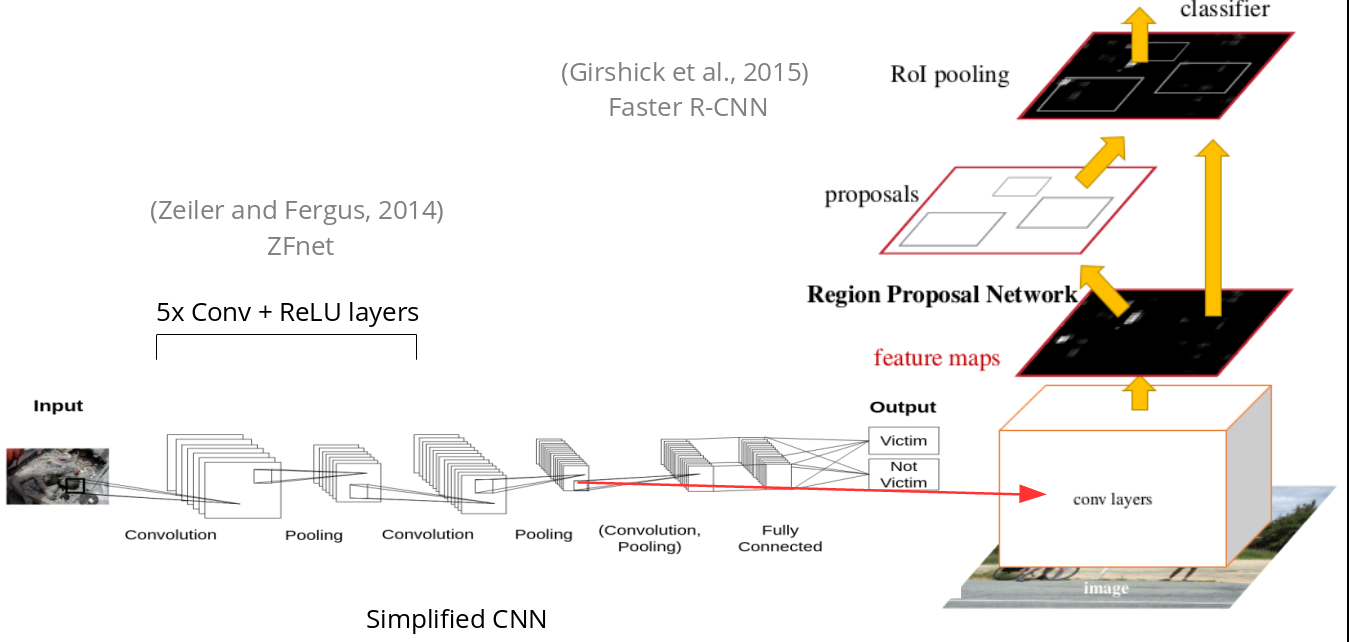
\includegraphics[width=\textwidth]{struktur_rcnn}
  \caption{Faster R-CNN untuk Korban Bencana Alam}
  \label{fig:struktur_rcnn}
\end{figure}s

\subsection{ Penjelasan masing masing layer (yang di ipynb)}
Lorem ipsum dolor sit amet, consectetur adipiscing elit. Nullam ante quam, varius id tincidunt in, aliquet gravida felis. Praesent vehicula risus at pulvinar mattis. Duis feugiat diam ut massa euismod mollis. Maecenas tempus nisl diam, et sodales massa pharetra ut. Duis id ipsum ut dolor tincidunt euismod vitae sed odio. Duis tincidunt lorem ac leo mattis varius. Sed mollis metus nec tempor congue. Ut imperdiet dui ut ante mollis auctor. Suspendisse sit amet scelerisque sapien, in cursus nisl. Etiam egestas tellus mi, non fringilla justo ultricies at. Praesent eget ipsum porta, fermentum lorem sit amet, suscipit ligula. Nulla porttitor finibus neque nec sodales. Orci varius natoque penatibus et magnis dis parturient montes, nascetur ridiculus mus. Maecenas auctor quam ut justo accumsan, consequat eleifend massa imperdiet. Ut dictum eleifend justo, vitae pellentesque eros porta id.

\subsection{ Parameter (Learning rate dkk yang ada di option compile)}
Lorem ipsum dolor sit amet, consectetur adipiscing elit. Nullam ante quam, varius id tincidunt in, aliquet gravida felis. Praesent vehicula risus at pulvinar mattis. Duis feugiat diam ut massa euismod mollis. Maecenas tempus nisl diam, et sodales massa pharetra ut. Duis id ipsum ut dolor tincidunt euismod vitae sed odio. Duis tincidunt lorem ac leo mattis varius. Sed mollis metus nec tempor congue. Ut imperdiet dui ut ante mollis auctor. Suspendisse sit amet scelerisque sapien, in cursus nisl. Etiam egestas tellus mi, non fringilla justo ultricies at. Praesent eget ipsum porta, fermentum lorem sit amet, suscipit ligula. Nulla porttitor finibus neque nec sodales. Orci varius natoque penatibus et magnis dis parturient montes, nascetur ridiculus mus. Maecenas auctor quam ut justo accumsan, consequat eleifend massa imperdiet. Ut dictum eleifend justo, vitae pellentesque eros porta id.

\subsection{ Visualisasi Layer (Cara melihat visualisasi)}
Lorem ipsum dolor sit amet, consectetur adipiscing elit. Nullam ante quam, varius id tincidunt in, aliquet gravida felis. Praesent vehicula risus at pulvinar mattis. Duis feugiat diam ut massa euismod mollis. Maecenas tempus nisl diam, et sodales massa pharetra ut. Duis id ipsum ut dolor tincidunt euismod vitae sed odio. Duis tincidunt lorem ac leo mattis varius. Sed mollis metus nec tempor congue. Ut imperdiet dui ut ante mollis auctor. Suspendisse sit amet scelerisque sapien, in cursus nisl. Etiam egestas tellus mi, non fringilla justo ultricies at. Praesent eget ipsum porta, fermentum lorem sit amet, suscipit ligula. Nulla porttitor finibus neque nec sodales. Orci varius natoque penatibus et magnis dis parturient montes, nascetur ridiculus mus. Maecenas auctor quam ut justo accumsan, consequat eleifend massa imperdiet. Ut dictum eleifend justo, vitae pellentesque eros porta id.
